%==============================================================================
\chapter{Simulation}
\label{sec:sim}
%==============================================================================

As this thesis is about estimating the performance of the PINGU detector before
it is actually built, the estimate has to be based on simulations. In this
chapter, the simulations used to generate the results reported in
Chapter~\ref{sec:ana} will be described in detail.

The chapter, as the simulation process, is divided into two sections.
In Sec.~\ref{sec:sim_MCchain} the existing and well-established IceCube Monte
Carlo (MC) chain will be discussed, which has been adopted for PINGU
simulations.
Here, individual neutrino events are generated and their output of Cherenkov
photons is modelled. After propagating the photons through the ice, the
resulting pattern of triggered optical modules is processed through the standard
reconstruction and event
selection specified in Secs.~\ref{sec:EvtReco} and \ref{sec:EvtSel},
respectively. The outcome of this event-by-event MC, \ie the effective
areas, reconstruction resolutions, and particle identification efficiencies for
all neutrino flavours, are then used as input for the second part of the
detector simulation.

The Parametric PINGU Analysis, \papa in short, was written specifically for the
rapid analysis of PINGU's neutrino mass hierarchy sensitivity including a
variety of systematic parameters. Since propagating these through the full
MC chain would be too time-consuming, an effective detector
simulation was implemented. Instead of operating on individual events,
the expected event distributions are generated directly, based on the detector
performance retrieved from the MC data. \papa will be described in
detail in Sec.~\ref{sec:papa}.

%==============================================================================
\section{The IceCube/PINGU Simulation Chain}
\label{sec:sim_MCchain}
%==============================================================================

\subsection{Event Generation}
\label{sec:MC_genie}

The first step in the MC chain is to model the interaction of an incoming
neutrino with a target nucleus in the ice and the resulting final state, the
so-called
event generation. In the dedicated PINGU MC, this is carried out using the
GENIE (Generates Events for Neutrino Interaction Experiments \cite{GENIE})
software package. This is already the first modification of the standard
IceCube MC chain, where NuGen \cite{NuGen}, an IceCube-specific neutrino
generator, is the default. NuGen is laid out for high-energy neutrino
events where only deep inelastic scattering has to be considered as an
interaction process. In PINGU, however, the low GeV energy range contains the
interesting signal for an oscillation measurement, and here the complex
interplay between
quasi-elastic and deep-inelastic scattering as well as resonant processes has
to be taken into account (see Sec.~\ref{sec:XsecsGeV}). Since GENIE puts much
effort into modelling especially this energy range with great care and
validating it against experimental results, it is the natural choice for
generating PINGU events.

GENIE starts off with an isotropic flux of neutrinos of a given flavour
following a user-defined power-law distribution in energy (usually $\propto
E^{-1}$ or $E^{-2}$ for PINGU MC \cite{PINGU_MC}) on the surface of a
cylindrical generation volume well encompassing the full IceCube detector. Any
generated neutrino passing through the interaction volume, which is fully inside
the generation volume but still contains the detector as a whole, is forced to
interact inside this volume. The interaction type is chosen randomly from the
ones that are allowed and the event is assigned a weight $\mathcal{W}_i$
proportional to the particular interaction probability, taking into account the
generated energy spectrum. This weighting strategy makes it possible to
re-weight the generated events to any desired incoming flux $\Phi(E, \theta,
\varphi)$ later on. Then the actual weight is simply given by
\begin{equation}
 w_i = \frac{\Phi(E_i, \theta_i, \varphi_i)\,\mathcal{W}_i}{N_\mathrm{evts}}
  \quad, \label{eqn:reweight}
\end{equation}
where $N_\mathrm{evts}$ is the total number of simulated events.

After the interaction mechanism has been determined, the interaction itself is
modelled in detail and all involved particles, from the initial neutrino and
nucleus over possible intermediate states to the final (meta-)stable particles
like pions or muons, are stored inside an \texttt{I3MCTree} object for further
processing. The reference to a tree comes from the fact that this object has
the structure of a multiply nested list, where every particle is the root of a
sub-tree (or branch) holding the particles created in its decay. The particles
are characterised by their identities, positions, four-momenta, and state (such
as `initial', `intermediate', or `final').
Additional GENIE-specific information such as the number of generated events,
$N_\mathrm{evts}$, the size of the interaction volume, and others, are kept as
an \texttt{I3MCWeightDict} object.

\subsection{Particle Propagation}
\label{sec:MC_propagation}

The \texttt{I3MCTree} generated by GENIE is handed off to the mmc
module \cite{mmc}, which propagates the final state particles in the tree as
well as possible secondaries created in their decay through the ice until they
have deposited all their energy. The particles involved here are mainly 
produced in the electromagnetic and hadronic showers, as discussed in
Sec.~\ref{sec:XsecsGeV}. These are electrons, photons, and pions as well as
muons and taus. The \texttt{I3MCTree} is extended with the outcome of
mmc, additional information being stored as \texttt{MMCTrackList} and
passed on to another module called clsim \cite{clsim}.

clsim is then used to generate the Cherenkov photons produced by
the particles propagating through the ice. Therefore, every
particle is converted into a series of steps of constant velocity $\beta =
v/c$, over which Cherenkov photons are emitted according to
(\ref{eqn:FrankTammWvl}). Usually this process of photon generation is handled
by the Geant4 package \cite{Geant4_1, Geant4_2}, but can also be done using an
effective parametrisation as well.

These photons are then propagated through the ice until they either get absorbed
or hit a DOM. Since photon propagation is a process that can well be run in 
parallel by multiple computation threads, clsim uses the publicly
available OpenCL library \cite{OpenCL} to outsource the calculations to GPUs,
resulting in a significant speedup compared to a simulation on CPUs. The photons
that have hit and launched a DOM, taking into account its angle- and
wavelength-dependent quantum efficiency (see Fig.~\ref{fig:DOMeff}), are stored
in a \texttt{I3MCHitSeriesMap}. This object contains the registered photons and
the corresponding DOM IDs; other information such as the parent particle,
wavelength, and position and angle of incidence on the hit DOM can be stored as
well. This information gets passed on to emulate the response of the actual
detector.

\subsection{Detector Response}
\label{sec:MC_detector}

\begin{figure}[ht]
\centering
  \subfloat[\label{fig:wvlQE}]
    {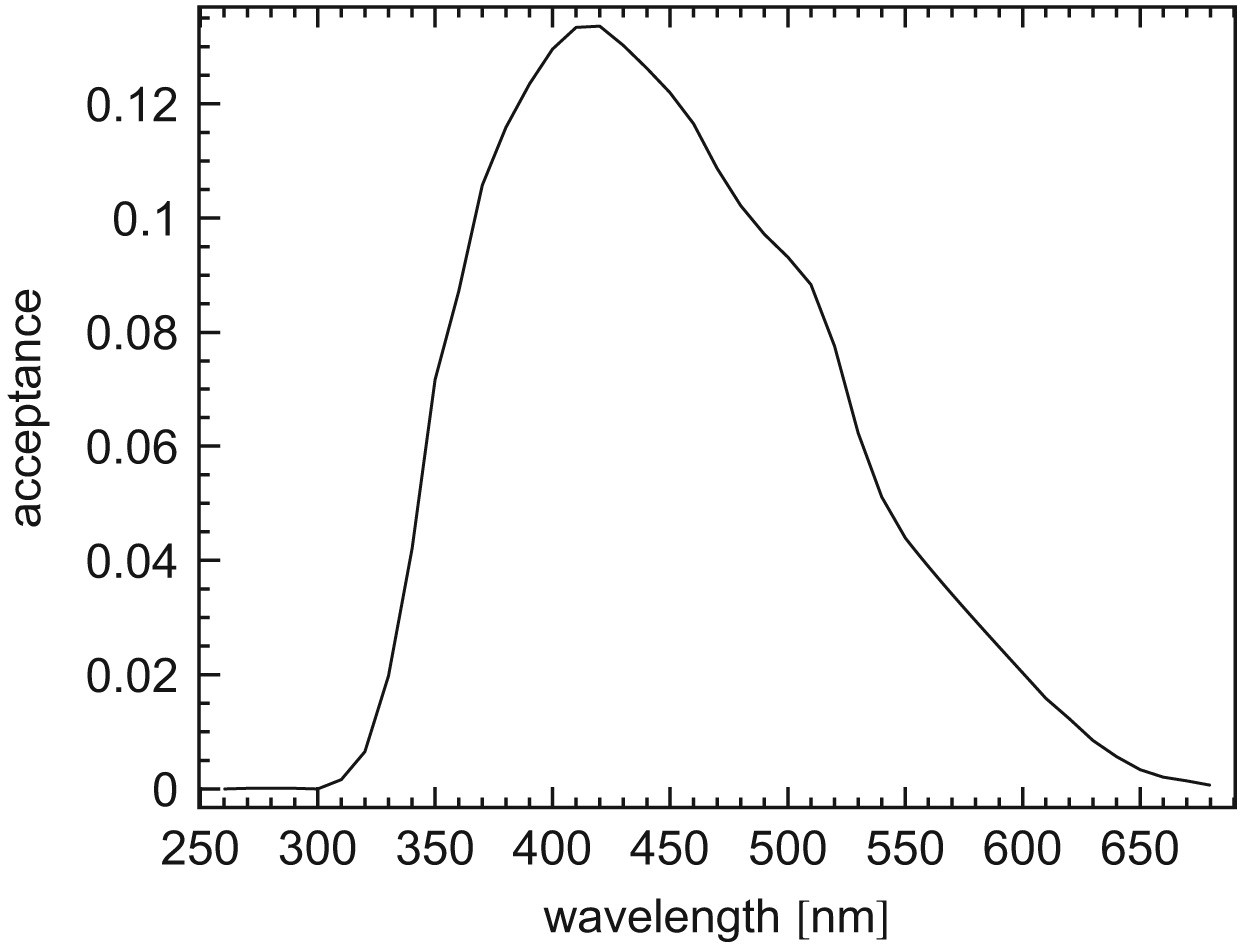
\includegraphics[width=0.5\textwidth]{DOM_wvl_QE}}%\qquad
  \subfloat[\label{fig:angEff}]
    {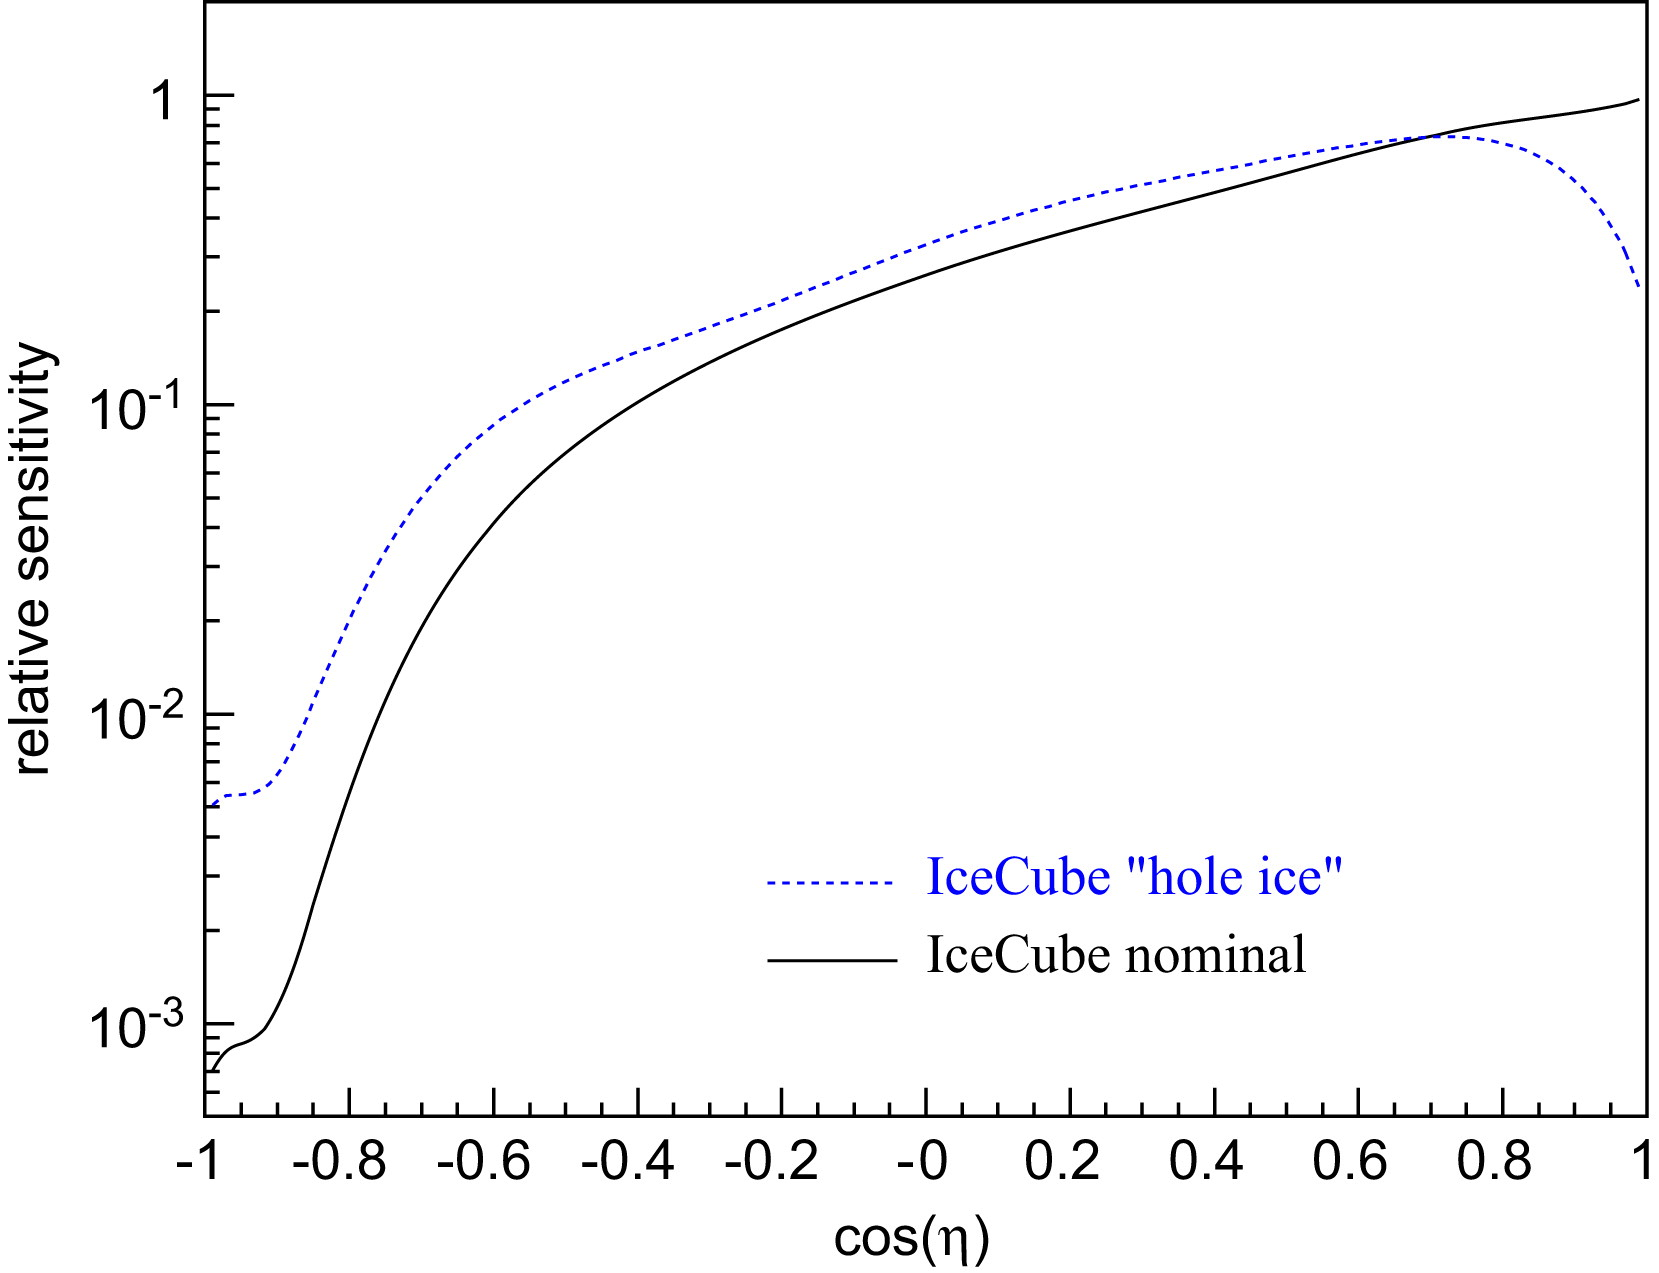
\includegraphics[width=0.5\textwidth]{DOM_ang_eff}}
  \caption{\protect\subref{fig:wvlQE} Quantum efficiency of the IceCube DOM
        as a function of the photon wavelength for head-on illumination.
        \protect\subref{fig:angEff} Normalised angular dependence of the
        acceptance for a ``bare'' DOM and a DOM inside ``hole ice'', with
        $\eta$ denoting the angle towards the centre of the PMT front. Plots
        taken from \cite{Dima}.}
\label{fig:DOMeff}
\end{figure}

In PINGU simulations, all DOMs are represented by an identical copy of the
standard DeepCore DOM, having a 35\,\% higher quantum efficiency than the
IceCube DOM (see Sec.~\ref{sec:ICDOM}). This is only an approximation of the
actual PINGU DOM, which currently only exists as a prototype, however it has
already become clear that especially the digitisation process will be
simplified. Yet as the PDOM design is not finalised, the DeepCore DOM is the
closest approximation at hand.

Before the response of the DOMs gets evaluated, noise hits from both thermal
electronic noise as well as radioactive decays inside the DOM and the
accompanying scintillation and fluorescence light are added to the
\texttt{HitSeries} with the vuvuzela module \cite{vuvuzela}. Then the
DOMLauncher module \cite{DOMLauncher} is called to generate the actual DOM
output.

\begin{figure}
\centering
  \subfloat[\label{fig:PMTjitter}]
    {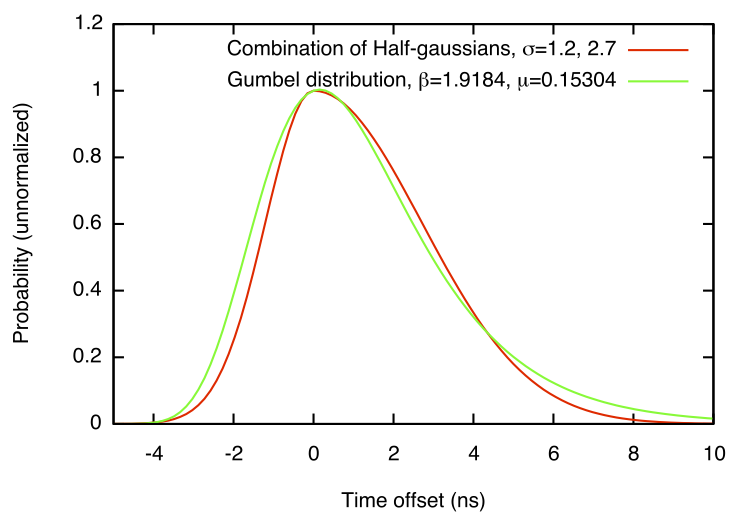
\includegraphics[width=0.5\textwidth]{Jitter_Parameterization}}%\qquad
  \subfloat[\label{fig:SPEcharge}]
    {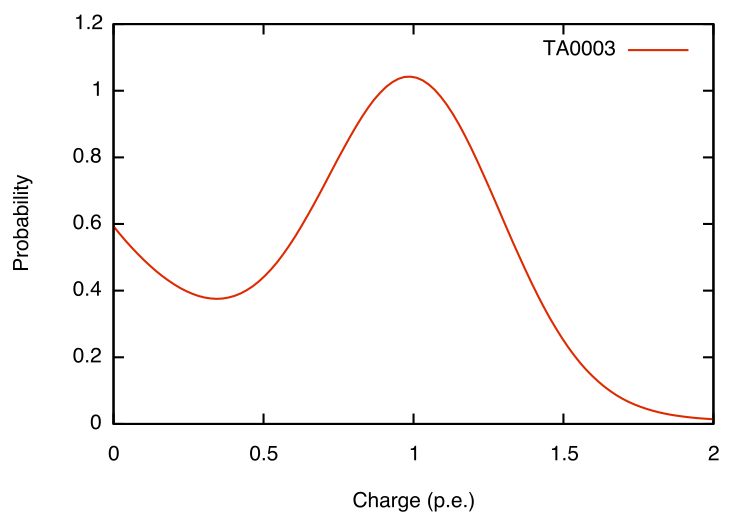
\includegraphics[width=0.5\textwidth]{TA0003}}
  \caption{Parametrisation of \protect\subref{fig:PMTjitter} the PMT transit
       time jitter distribution (in green) and \protect\subref{fig:SPEcharge}
       the single photo-electron charge distribution as used by the
       \texttt{PMTResponseSimulator}. Plots taken from \cite{PMTRes}.}
\label{fig:PMTRes}
\end{figure}

The DOMLauncher first calls the PMTResponseSimulator submodule \cite{PMTRes} to
convert the single photo-electron produced at the PMT cathode by a DOM hit to a
charge pulse entering the DOM electronics. Here, the PMT transit time jitter is
applied, which takes into account that there is a spread in the time needed by
the electron
avalanche developing on the PMT dynodes to pass through all amplification
stages. This distribution is shown in Fig.~\ref{fig:PMTjitter}. The
distribution of the amount of charge generated by a single photo-electron is
dominated by a Gaussian, per construction centred at the charge equivalent of
one photo-electron, but also contains a exponentially decreasing component of
small-amplitude pulses, as shown in Fig.~\ref{fig:SPEcharge}.

Once the main photon pulse has been processed, secondary effects like pre-,
late, and after-pulses are added. These result from photons hitting the first
dynode instead of the photocathode, scattered avalanche electrons hitting the
same dynode twice, and ionised residual gas atoms drifting onto the
photocathode, respectively, and are offset by a specific time window from the
main bunch of photo-electrons, but causally connected. Finally, saturation
effects are taken into account, which have to be considered for events of very
high energy or with an interaction vertex in the close proximity of a single
DOM.

The full PMT charge output as a function of time, or ``waveform'', is then
passed to the main DOMLauncher module, which simulates the processing and
digitisation of the raw PMT signal on the DOM main board \cite{DOMLauncher}.
First
a discriminator threshold and local coincidence logic are applied, deciding
whether a waveform gets digitised based on its strength and coincidence with a
hit on a neighbouring DOM. These steps will be removed in the actual PDOM since
advances in technology allow a continuous readout of the PMT waveform by a
single ADC instead of the multiple parallel ATWDs \cite{PDOM_Aachen}. Finally,
electronic noise in the digitisers and uncertainties in the time calibration are
added and a digitised representation of the waveform is created, which can then
be injected in the actual reconstruction chain described in
Secs.~\ref{sec:EvtReco} and \ref{sec:EvtSel}.

%==============================================================================
\section{The \papa Code}
\label{sec:papa}
%==============================================================================

\subsection{Idea}
\label{sec:sim_idea}

As already discussed in Sec.~\ref{sec:PINGUosc}, the primary science goal of
PINGU is the determination of the neutrino mass hierarchy, imprinted on the
oscillation probability pattern of the atmospheric electron and muon neutrinos
travelling through the Earth's matter potential. Observing such a small effect
requires a precise high-level analysis and a detailed knowledge of the detector 
performance. 

The observable in the mass hierarchy analysis is the distribution of arriving 
neutrinos in the ($E$, \coszen) plane. The shape of this distribution is 
determined not only by the mass hierarchy, but also by the true values of the 
other neutrino mixing parameters as well as the reconstruction efficiency and
precision of the detector. All those quantities---and especially their 
uncertainties---have to be taken into account estimating the significance 
which PINGU can determine the mass hierarchy with.

The standard procedure to account for systematic uncertainties in IceCube is a 
brute force approach, where the parameters in question get increased and 
decreased by an amount corresponding to the estimated uncertainty. Then the 
simulation is re-run for each setting and the sensitivity re-evaluated. For the 
mass hierarchy measurement with PINGU, however, this strategy is not 
applicable. The reason for this is that in IceCube analyses usually only search 
for the existence of events passing a certain set of selection criteria---it is 
a detection experiment, where systematics in general have a much less severe 
impact compared to the search for a pattern in a large amount of data. Here, 
correlations between the systematics have to be taken into account as well, 
while in IceCube they can be considered independent. Additionally, the number 
of relevant systematic parameters is much higher for PINGU, since in IceCube 
oscillations are not measured in such detail, and the detector itself is much
better understood as it is
already operating and hence could be studied and modelled in great detail.

Thus, re-running the whole simulation chain for all possible combinations of
these parameters---which will be treated in detail in
Sec.~\ref{sec:systematics}---is not feasible in a reasonable amount of time.
This is especially true since a comparatively large number 
of MC events---in the order of $10^6$---is needed to make a reliable estimate of
the sensitivity. In case of insufficient MC events, statistical fluctuations
will exceed the strength of the imprinted mass hierarchy pattern and bias the
calculated significance towards high values, as it will be demonstrated in
Sec.~\ref{sec:results_mcstats}.

The basic idea how to overcome this fundamental problem is to move away from an 
event-by-event MC simulation and simulate the event histograms in
($E,\,\coszen$) directly, based on parametrisations of the relevant detector 
quantities that are extracted from MC data. This is much faster than filling 
the histograms with individual events and has the benefit of quasi-infinite 
statistics since the parametrisations will in general be smooth functions, 
resulting in inherently smooth distributions. This strategy has been 
implemented in the \papa code, which will be described in detail in the
following section.

A certain amount of MC events is still needed to produce the parametrisations 
that are the input to \papa, however it has been found during the
parametrisation process that about 20,000 events 
per neutrino flavour are sufficient to get stable fit results. This is at least
a factor of ten less than the number of events required to reach a stable 
result in Sec.~\ref{sec:results_mcstats}. Also, the MC simulation does not need
to be re-run for the different settings of the systematic parameters, as they
are tuned within \papa.

\subsection{Implementation}
\label{sec:papa_code}

The \papa source code is available in the IceCube subversion repository 
\cite{papa_code}, with a detailed manual and version history maintained at the 
IceCube wiki pages \cite{papa_wiki}. It is written entirely in the python 
programming language \cite{python} and relies heavily on the numpy and scipy
packages for numerical and scientific computing \cite{numpy, scipy}, with
graphical output functionality based on the matplotlib library
\cite{matplotlib}.

\begin{figure}
\centering
 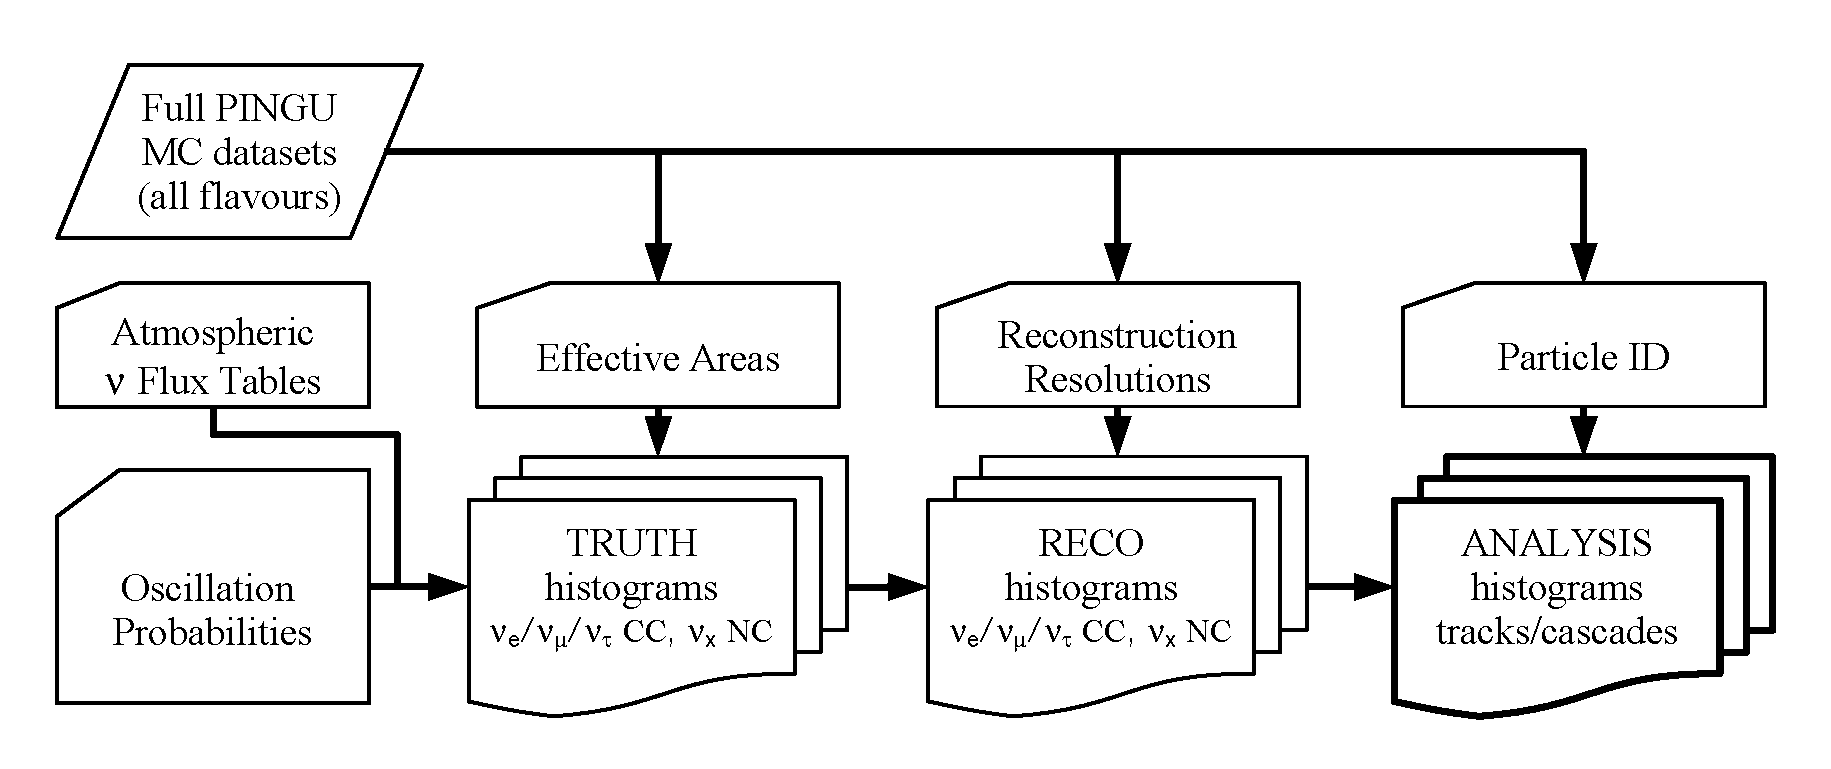
\includegraphics[width=\textwidth]{PaPA_flowchart}
 \caption{Flow chart of the \papa simulation chain}
\label{fig:papa_flowchart}
\end{figure}

\papa employs a staged processing procedure following the logical ordering and 
emulating the effects of the multiple physics processes that are involved in 
the actual measurement, as illustrated in Fig.~\ref{fig:papa_flowchart}. The 
code itself is split into two main parts that are run separately. The first 
part is the \texttt{PhysicsSimulation}, responsible only for the calculation of 
neutrino oscillation probabilities. In the second part of \papa---the 
\texttt{DetectorSimulation}---the actual event histograms as observed in PINGU 
are calculated from the oscillation probabilities and detector settings.


\subsubsection{\texttt{PhysicsSimulation}}

In the physics simulation the neutrino oscillation probabilities in
the full three-flavour mode including matter effects are calculated, using
either NuCraft \cite{NuCraft} or AtmoWeights \cite{AtmoWeights} and assuming
the Preliminary Reference Earth Model (PREM) \cite{PREM} for the Earth's density
profile. The difference between the two software modules is that NuCraft is more
versatile in the sense that it
can include the oscillation into sterile neutrino flavours, model the
generation heights of the neutrinos in the Earth's atmosphere in more detail,
and handle a varying electron density in the Earth while in AtmoWeights this
value is fixed to 0.5 electrons per nucleon. On the other hand, AtmoWeights is
much faster. After checking consistency of the two softwares to the sub-permill
level given the same input, AtmoWeights has been selected for the baseline
analysis due to its higher speed. The additional options provided by NuCraft are
not essential for the study of the neutrino mass hierarchy.

The oscillation probabilities are calculated for $\nu_e$, $\bar\nu_e$, $\nu_\mu$
and $\bar\nu_\mu$ injection, such that twelve histograms of oscillation
probabilities are obtained:
\begin{itemize}
 \item $P(\nu_\alpha \to \nu_e/\bar\nu_e)$
 \item $P(\nu_\alpha \to \nu_\mu/\bar\nu_\mu)$
 \item $P(\nu_\alpha \to \nu_\tau/\bar\nu_\tau)$
\end{itemize}
with $\nu_\alpha \in \left[\nu_e,\bar\nu_e,\nu_\mu,\bar\nu_\mu\right]$. Since
no CP violation is assumed\footnote{It has been checked that if CP violation
existed, it would not be detectable with PINGU in any case.}, there is no
oscillation between neutrinos and antineutrinos.

% The relevant parameters for this step in the simulation chain are the physical
% ones, i.\,e.\ the mixing angles, mass splittings, hierarchy, and for
% implementation reasons also the energy scale (see below).

To properly sample the fast oscillations at low energies, \papa can be set up
to oversample by given factors in energy and zenith. This means that every
point at which the oscillation probabilities are calculated is replaced by a
number of evenly spaced points in the vicinity, and the resulting probabilities
are averaged over. If no oversampling is applied, the values at the bin
centres are used.
% For our calculations, we used oversampling factors of eight in energy and two in
% zenith.

As mentioned above, the calculation of the oscillation probabilities is the 
most time-consuming part of the simulation as here the Schr\"odinger equations 
for full three-flavour oscillations in a varying matter 
potential (see Sec.~\ref{sec:matter_osc}) have to be solved numerically.

% differential equations for neutrino propagation need to be solved numerically.
To get all oscillation probabilities needed for a full analysis, the three
relevant oscillation parameters \dm{31}, \thet{23}, and \thet{13} as well as the
energy scale (see Sec.~\ref{sec:systematics}) have to be varied independently at
15 test points each. This typically takes several hours on a single CPU whereas
with NuCraft this goes up to a few days. Fortunately, the fiducial settings for
the oscillation parameters do not change when the detector parametrisation
changes, meaning that the oscillation probabilities only have to be calculated
once and can then be re-used for different detector settings.


\subsubsection{\texttt{DetectorSimulation}}

In the detector simulation the pure oscillation probabilities calculated in the
physics simulation are converted into an actual detector response, taking into
account all detector related parameters. It consists of three major steps, as
depicted by the flow chart in Fig.~\ref{fig:papa_flowchart}. At each step, a 
histogram in ($E$,\,\coszen) will be produced for every event signature that has 
to be considered at the respective stage. Event
histograms at all simulation stages are shown in Fig.~\ref{fig:SimSteps}.

\begin{figure}
 \centering
 $\begin{array}{cc}
   \mathrm{Tracks} &
   \mathrm{Cascades}\\
   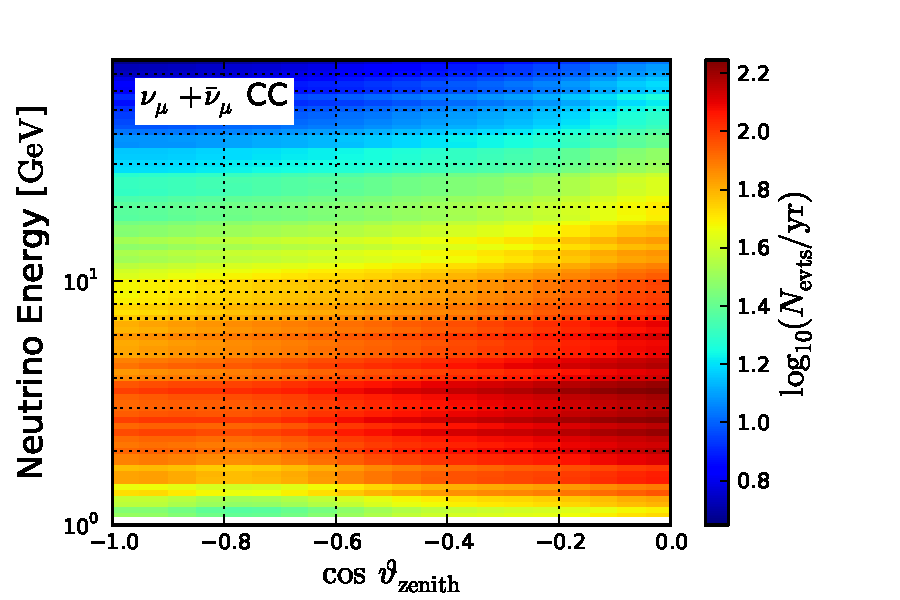
\includegraphics[width=0.48\columnwidth]{1_un_oscillated_trck} &
   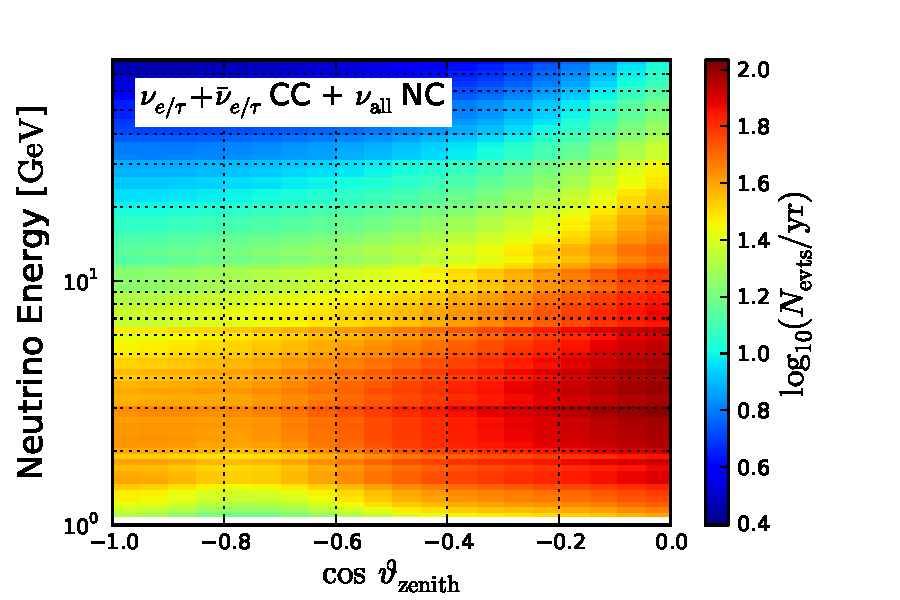
\includegraphics[width=0.48\columnwidth]{1_un_oscillated_cscd}\\
   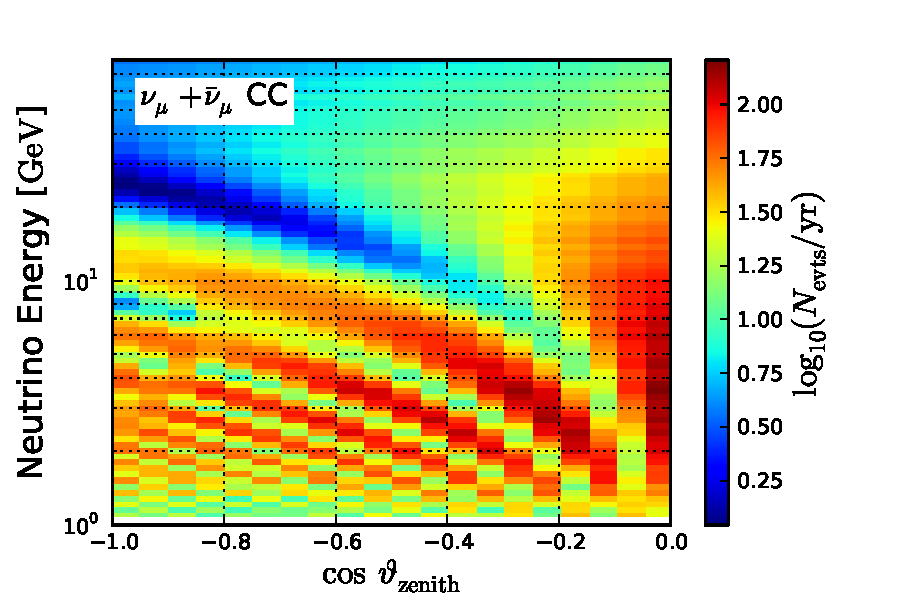
\includegraphics[width=0.48\columnwidth]{2_oscillated_trck} &
   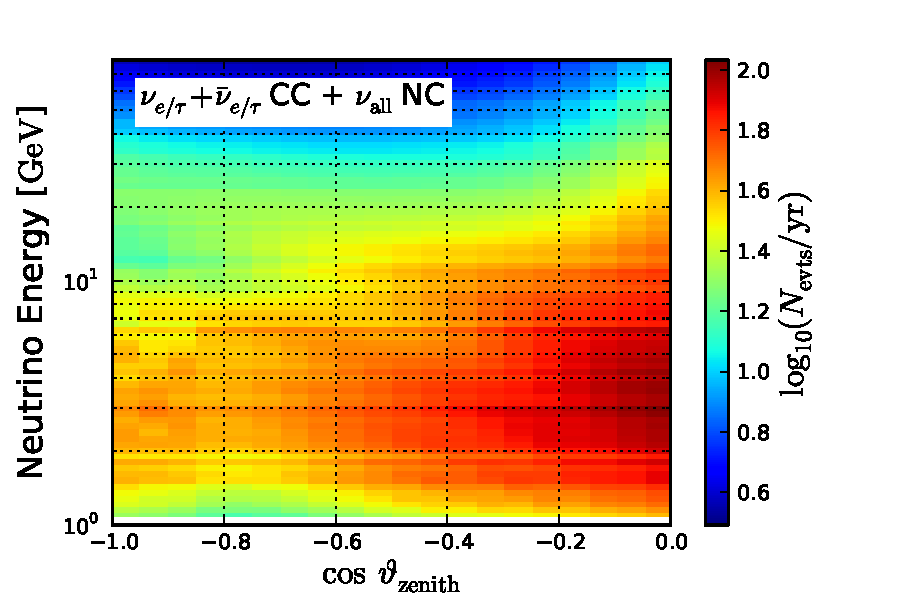
\includegraphics[width=0.48\columnwidth]{2_oscillated_cscd}\\
   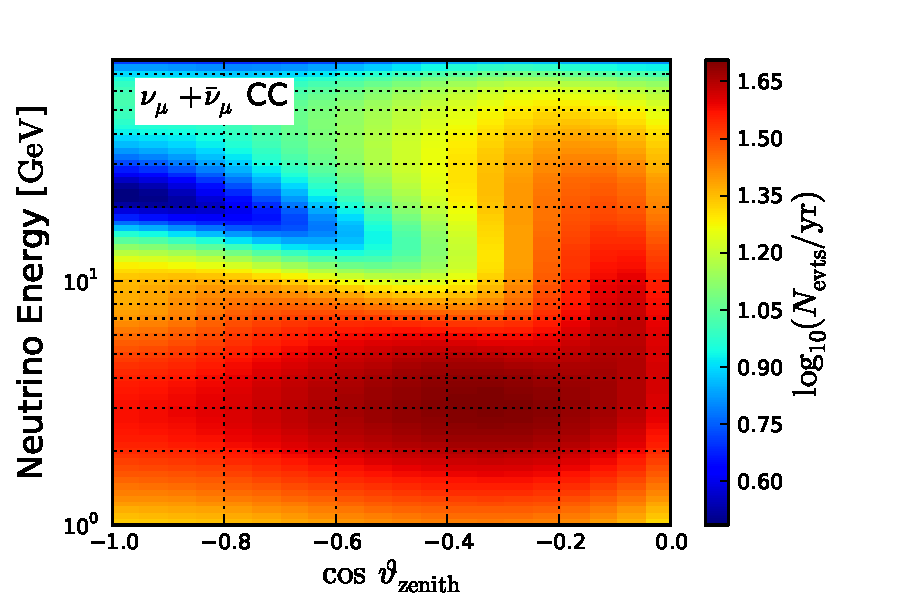
\includegraphics[width=0.48\columnwidth]{3_reconstructed_trck} &
   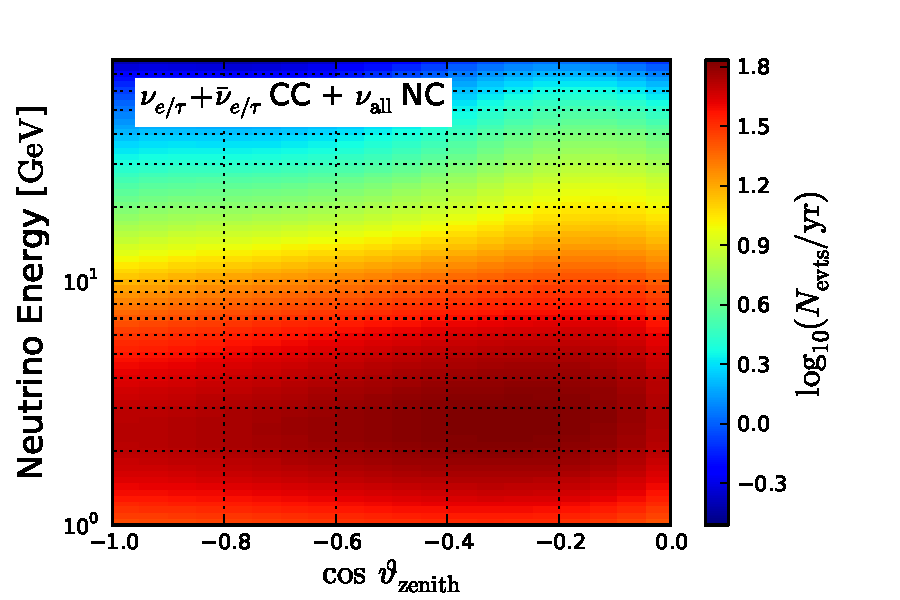
\includegraphics[width=0.48\columnwidth]{3_reconstructed_cscd}\\
   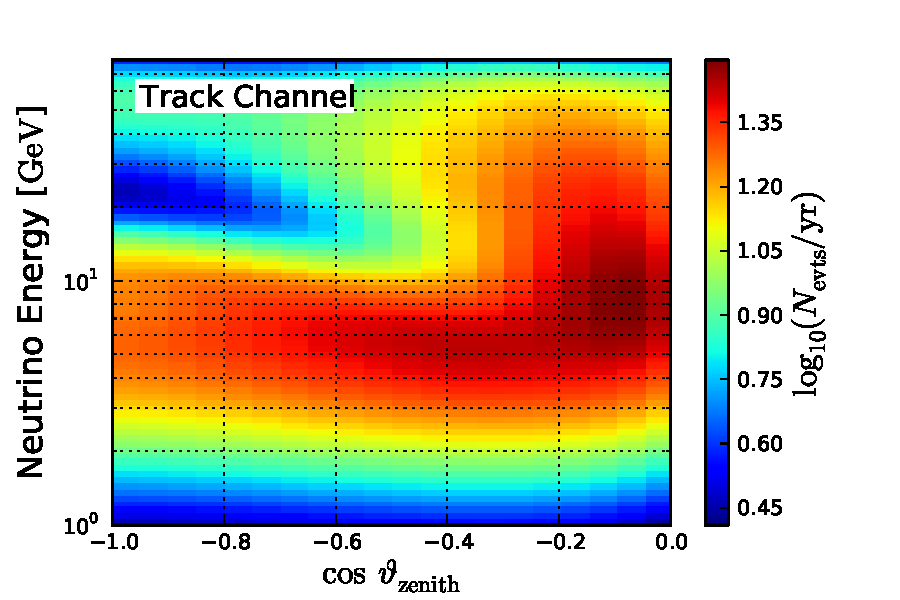
\includegraphics[width=0.48\columnwidth]{4_classified_trck} &
   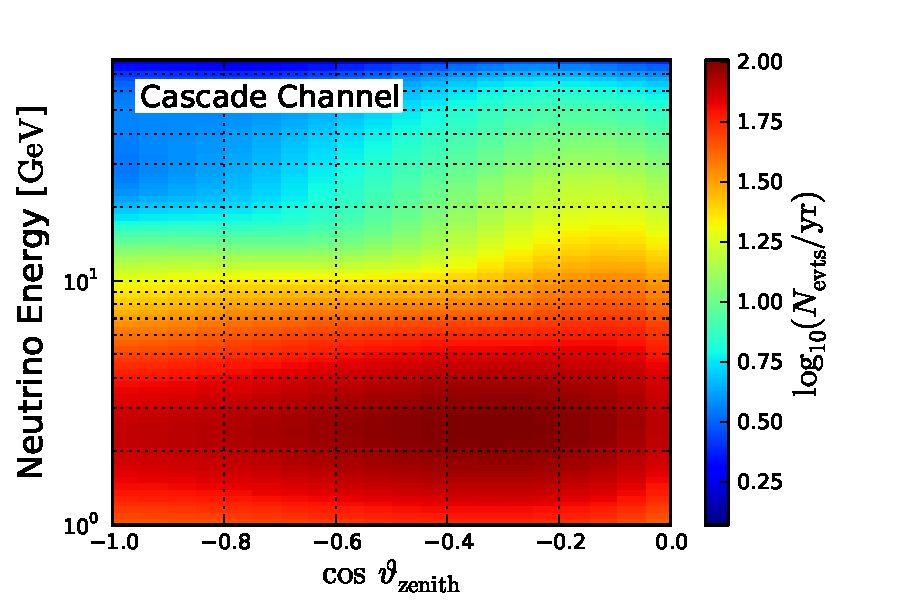
\includegraphics[width=0.48\columnwidth]{4_classified_cscd}
  \end{array}$
 \caption{Event counts in one year of PINGU lifetime at the different
  simulation stages, assuming normal mass hierarchy. From top to bottom: 
  Truth Histograms without and with oscillations, Reconstructed and Analysis 
  Histograms. The variables are true neutrino energy and direction for the
  upper two rows of histograms and reconstructed energy and direction for the
  bottom ones. For details, refer to the text.}
 \label{fig:SimSteps}
\end{figure}

\paragraph{Truth Histograms}

The first step is to calculate the true rates of events triggering the
detector. Therefore, spline fits are generated for the azimuth-averaged
atmospheric neutrino flux tables by Honda et al.\ \cite{Honda,
HondaSP}, from which then the fluxes for $\nu_e/\bar\nu_e$ and
$\nu_\mu/\bar\nu_\mu$ can be retrieved. These fluxes are multiplied by the
oscillation probabilities $P(\nu_\alpha \to \nu_\beta)$ calculated in the
physics simulation to obtain the flux for each neutrino flavour at the
detector:
\begin{equation}
 \Phi_{\beta,\,\mathrm{det}} =
   \sum_\alpha \Phi_{\alpha,\,\mathrm{atm}}\ P(\nu_\alpha\to\nu_\beta)
 \label{eqn:detetor_flux}
\end{equation}

To obtain event rates, the neutrino fluxes are then multiplied by the effective
areas of PINGU for 
$\nue/\nuebar$, $\numu/\numubar$ and $\nutau/\nutaubar$ CC interactions as well 
as $\nu_X/\bar\nu_X$ NC---the four different interaction channels---after
background rejection cuts (cf.\ Sec.~\ref{sec:EvtSel}). The effective area, a
function of neutrino energy and zenith direction, is defined as the collection
area an ideal detector identifying every neutrino passing through it would need
to have in order to achieve the same event rate as PINGU. For a given
interaction channel, it can be calculated according to
\begin{equation}
 \aeff(\mathrm{channel}) = \sum_\mathrm{target} N_\mathrm{target}\ 
   \sigma_{\mathrm{target},\,\mathrm{channel}}\ \epsilon_\mathrm{channel} \quad,
\end{equation}
summing over the possible targets, protons and neutrons. Here,
$N_\mathrm{target}$ stands for the total number of the respective targets
inside the detector volume, $\sigma_{\mathrm{target},\,\mathrm{channel}}$ is
the interaction cross section in the given channel, and
$\epsilon_\mathrm{channel}$ is the efficiency which interactions occurring
inside the detector actually pass the triggering, reconstruction, and event
selection process with. Although the selection efficiency is usually of the 
order of 80\,\% \cite{cutsV5}, see Fig.~\ref{fig:selection_eff}, the effective 
area is much smaller than the geometrical
size of the detector as the interaction cross sections for neutrinos are
extremely small (see Sec.~\ref{sec:Xsecs}). Hence, most neutrinos pass the
detector without any interaction.

The number of expected events per lifetime $t$ in a given channel can, thus, be
calculated by
\begin{eqnarray}
 N_\mathrm{\nu_\alpha\ \mathrm{CC}} &=&
   \aeff(\nu_\alpha\ \mathrm{CC})\ \Phi_{\alpha,\,\mathrm{det}}\ t 
   \label{eqn:evtrate_CC} \\
 N_{\nux\ \mathrm{NC}} &=&
   \aeff(\nux\ \mathrm{NC}) \sum_\alpha \Phi_{\alpha,\,\mathrm{det}}\ t
   \label{eqn:evtrate_NC} 
\end{eqnarray}
for the three charged and one neutral current channels, respectively.
Finally, the histograms for neutrinos and anti-neutrinos in the same
interaction channels are added since PINGU will not be able to distinguish
between them. Also in terms of reconstruction quality and flavour
identification (see below) there is no difference between neutrinos and
anti-neutrinos. 

Since both the fluxes and the effective areas are functions of $E$ and \coszen,
the result of this simulation step are four 2D histograms, one each for the
four channels $\nue+\nuebar$ CC, $\numu+\numubar$ CC, $\nutau+\nutaubar$ CC, and
$\nux+\nuxbar$ NC, examples of which are shown in the second row of
Fig.~\ref{fig:SimSteps}.

\paragraph{Reconstructed Histograms}

In the next step, event reconstruction is applied to the histograms that up
to now contain \emph{true} neutrino energies and directions. This is done by
smearing
the true histograms with a kernel\footnote{A \emph{smearing kernel} can be
interpreted as a binned point spread function.} whose shape depends on the true
energy and zenith angle of the event, i.\,e.\ the position in the histogram.
There are two different ways how these kernels can be handed over to \papa:

\begin{enumerate}[(a)]
 \item Parametrised point spread functions.\\ These have to be fitted from MC
  data and generally take the form of a double Gaussian for both energy and
  $\cos\vartheta$ to properly account for the tails of the reconstruction 
  distributions:
  \begin{equation}
   \mathrm{PSF} = (1-f)\cdot \exp\left(-\frac{(x-\mu_1)^2}{\sigma_1^2}\right)
                  + f\cdot \exp\left(-\frac{(x-\mu_2)^2}{\sigma_2^2}\right)
   \label{eqn:reco_param}
  \end{equation}
  The five parameters (two mean values $\mu_i$, two widths $\sigma_i$, and the
  relative normalisation $f$) are supplied to the code as a function of true
  neutrino energy.\\
  Here it can happen that events are ``leaking'' out of the histograms. At
  the edges of the energy range this effect can be neglected since the event
  rates are small anyways (due to low flux/small effective area). In the
  directional dimension, losing events at the horizon is accepted since
  mis-reconstructed events will be also be lost in the real experiment due to
  cutting the analysis at the horizon. Events that would be lost at the zenith
  are reflected back into the histogram, as events migrating ``over the
  zenith'' will flip the sign of their azimuth angle (which is irrelevant) and
  move back to larger values of the zenith angle.
 \item Tabulated point spread functions.\\ If the MC statistics is sufficient,
  \ie in the order of $10^6$ events per flavour, the resolutions can be
  retrieved directly from the MC data. This means creating a 4D histogram of
  true vs.\ reconstructed ($E$, \coszen), which is equivalent to
  the individual smearing kernel for each bin in true ($E$, \coszen).
  \end{enumerate}
Option (a) is used primarily in this study, since for the PINGU geometry
V36 that is the baseline for all analyses, the amount of MC events is
insufficient for option (b). Also, the parametrised reconstruction resolutions
make it possible to investigate the effects of an improved resolution within a
well-defined metric in Sec.~\ref{sec:wom_effect}.
For the earlier PINGU geometry V15, however, enough MC events exists to
follow option (b) for the event reconstruction stage.
This is reported on in Sec.~\ref{sec:results_mcstats}, where also the effect
that an insufficient MC sample has on the calculated NMH sensitivity is
demonstrated.

Example histograms after the reconstruction stage---still in the four
interaction channels already present after the previous stage---are shown in
the third row of Fig.~\ref{fig:SimSteps}. However one has to keep in mind that
now the variables have changed from \emph{true} to \emph{reconstructed}
neutrino energies and directions. The reconstructed neutrino energy is given by
the sum of the deposited energies of the cascade and track as fitted by
HybridReco/MultiNest. The reconstructed direction comes from the same
algorithm, where track and cascade are assumed to be aligned (cf.\
Sec.~\ref{sec:reco_multinest}).

\paragraph{Analysis Histograms}

Up to now, the histograms are still divided into the four ``effective flavour''
channels, \nue, \numu, \nutau CC and \nux NC, each including
anti-neutrinos. The final step in the detector simulation is to apply the
particle flavour identification (PID). However, current tools for particle ID
can only distinguish events with an outgoing muon signature (only present in
$\nu_\mu$ CC interactions), which are classified as tracks, from other events
(cascades), as already described above (cf.\ Sec.~\ref{sec:cuts_PID}).

So for every interaction channel, two analytic functions of the neutrino
energy have to be supplied to \papa, giving the probabilities of identifying a
neutrino of that channel and energy as either track or cascade. If those two
probabilities add up to less than one, the remaining events are assigned to an
``unidentified'' channel that can be used for the analysis as well.

For the baseline settings (Sec.~\ref{sec:sim_input}), the PID is a binary
decision, meaning that there are no unidentified events. In
Sec.~\ref{sec:results_includeunkn}, the effects of an event selection producing
cascade and track samples of higher purity plus a set of unidentified events
will be discussed.

After this final stage, all key features of a real experiment (triggering,
event selection, reconstruction, and flavour identification) have been taken
into account, and the analysis histograms are the best estimate of the outcome
of an actual PINGU physics run. Example histograms after this final step, also
referred to as analysis histograms, are shown in the bottom row of
Fig.~\ref{fig:SimSteps} and will also be used throughout Chapter \ref{sec:ana}
to illustrate the various effects studied.


\subsection{Systematic Parameters}
\label{sec:systematics}

The main benefit of the fast simulation provided by \papa is that it makes the
inclusion of
the many systematic parameters feasible, which are needed to correctly evaluate
the mass hierarchy significance. The parameters that were considered in this
thesis can be divided into two groups. The first one contains the \emph{physics}
parameters,
\ie the neutrino oscillation parameters: three mixing angles, two mass
splittings, the CP violating phase and of course the sign of the NMH. The best
fit values and priors for the mixing angles and mass splittings as listed in
Tab.~\ref{tab:fiducial_osc} are taken from \cite{Fogli}, assuming
inverted NMH as fiducial value. The CP violating phase $\delta_\mathrm{CP}$ is
set to a fiducial value of zero.
After having checked that their impact is negligible, the so-called solar mixing
parameters \dm{21} and \thet{12} as well as the CP phase will not be left free
to vary any more in order to save computation time.
% TODO: show that explicitly?

The mass hierarchy needs special treatment since it is a binary quantity,
yet the Fisher matrix formalism (see Sec.~\ref{sec:fisher}), which will be
used to quickly evaluate the simulation outcome, can only treat continuous
parameters. Thus the NMH
needs to be converted into a continuous variable. This is achieved by
calculating the oscillation probabilities assuming normal and inverted NMH once 
each and propagating both through the full \texttt{DetectorSimulation} chain 
as described in the previous section. Then a hierarchy parameter $0\leq h\leq1$
is introduced that allows for a continuous transition between normal (NH) and
inverted (IH) hierarchy:
\begin{equation}
 N(h) = h N_\mathrm{NH} + (1-h) N_\mathrm{IH}\quad,
 \label{eqn:hierarchy_parameter}
\end{equation}
where $N_\mathrm{NH}$ and $N_\mathrm{IH}$ are the expected number of events in
a given ($E,\,\coszen$) bin of the analysis histograms for normal and inverted 
mass hierarchy, respectively. All other oscillation parameters are kept at 
their fiducial values.

The rationale is that while in theory any value of $h$ other than $0$ or $1$ is
unphysical, in practice this definition allows to assess the deviation from the
physical points, as long as these are close to the fiducial values. It is such 
a measure of the hierarchy \textit{likeness}, similar to a
likelihood\footnote{It can also be interpreted as a measure of the orthogonal
distance of the hyperplanes in parameter spaces defined by normal and inverted
hierarchy}.
If no other parameters are present, this description is mathematically
equivalent to a bin-wise $\Delta\chi^2$ sum as defined in \cite{Akhmedov}, as 
it will be shown in Sec.~\ref{sec:fisher_hierarchy}.

The second set of parameters are related to the detector, which is commonly 
referred to as 
nuisance parameters. Most of them scale properties of the detector up or down, 
reflecting uncertainties in the knowledge of the detector performance. In 
several cases, however, they can be interpreted as theoretical uncertainties 
on, e.\,g., the neutrino cross sections or atmospheric flux tables. The
systematic parameters belonging to this class are, ordered according to their
entry point into the simulation chain:

\begin{description}
 \item[The energy scale $\mathbf{s_E}$] describes a potential scaling error
  in the assumed relation 
  between true and reconstructed neutrino energy. Such a mis-scaling, \ie
  a systematic under- or overestimation of the neutrino energy can be the 
  result of a wrong value for \eg PMT efficiency, absorption effects in the 
  ice model etc.\ that are used to reconstruct the neutrino events.
  It is implemented in a way that the true values of the energy bins that are 
  fed to the oscillation code are scaled \wrt the energy bins in the analysis 
  according to
  \begin{equation}
   E_\mathrm{true} = s_E\cdot E_\mathrm{ana}\quad.
  \end{equation}
  So the energy bins in the actual histograms remain unchanged, but the 
  oscillation minima and maxima do not appear at the expected energies. This 
  mimics the effect of a wrong energy scale in an actual analysis, since
  one would of course assume the energy scale to be correct. Note that in 
  \papa, the energy scale does affect neither the atmospheric flux calculations
  for the South Pole, as they are usually validated with existing IceCube
  data that would likely have the same energy mis-scaling as PINGU. Nor does it 
  change the
  effective areas, since their main feature, the energy threshold for 
  detecting a neutrino interaction, would scale in parallel with the energy bin 
  edges. Other accompanying effects, such as the overall normalisation of the 
  effective area, are absorbed in different systematic parameters. \\
  Although the energy scale is a detector-related parameter, it has to enter at 
  the \texttt{PhysicsSim\-ul\-ation} stage already as the rescaled energy bins 
  have to be passed on to the calculation of the oscillation probabilities. 
  Thus, it is the very first detector parameter in the simulation chain to be 
  accounted for.
 \item[The relative flux normalisation 
  $\mathbf{r_{\Phi,\,\nue-\numu}}$]
  represents the uncertainty on the relative contributions of \nue and \nuebar 
  vs.\ \numu and \numubar to the total flux of atmospheric neutrinos, which is 
  approximately 1:2. It is applied to the un-oscillated atmospheric neutrino
  fluxes (cf. (\ref{eqn:detetor_flux})) such that
  \begin{equation}
   \Phi_{\alpha,\,\mathrm{atm}}' = \Phi_{\alpha,\,\mathrm{atm}} \cdot 
      (1\pm r_{\Phi,\,\nue-\numu}) \quad,
  \end{equation}
  with positive sign for $\alpha=\nue$ or \nuebar and negative sign for 
  $\alpha=\numu$ or \numubar.
 \item[The effective area scale $\mathbf{s_{\aeff}}$] opens the
  possibility that the effective areas for all interaction channels scale
  differently with energy than assumed in the generation of the MC from where 
  they are extracted. It also partially compensates for a
  potential error in the spectral index of the atmospheric flux, since it
  effectively alters the total number of events per energy bin as a function of
  energy according to
  \begin{equation}
   \aeff' = \aeff\cdot\left(1+s_{\aeff}\cdot E\right)\quad.
  \end{equation}
 \item[The relative effective area normalisation 
  $\mathbf{r_{\aeff,\,\nu-\bar\nu}}$] for neutrinos and anti-neutrinos accounts 
  for a possible error in the relative normalisation of the neutrino-nucleon 
  cross sections for neutrinos vs.\ antineutrinos, which effectively alters the 
  effective areas\footnote{Inflicting this re-normalisation on the atmospheric 
  fluxes instead of the effective areas would have the same effect. Since the 
  effects are completely degenerate and uncertainties on the relative cross 
  sections are larger than on the relative fluxes, the flux normalisation is
  not treated as a parameter.}. The effective areas are then given by
  \begin{equation}
   \aeff' = \aeff \cdot (1\pm r_{\aeff,\,\nu-\bar\nu}) \quad,
  \end{equation}
  with the positive sign for neutrinos and the negative sign for antineutrinos. 
  Since the relative strength of neutrino and antineutrino interactions 
  governs the size of the NMH signal that can be observed with PINGU (see 
  Sec.~\ref{sec:PINGUosc}), this parameter is of particular importance.
 \item[The overall effective area normalisation $\mathbf{n_{\aeff}}$] 
  scales the effective areas for all channels independently of energy:
  \begin{equation}
   \aeff' = \aeff\cdot n_{\aeff}
  \end{equation}
  Since it just evenly increases the total number of events in all channels
  and, hence, is fully degenerate with the detector lifetime, it is not that
  interesting by itself. However, it is needed in combination with the relative 
  scalings mentioned above to effectively allow for separate scaling of one
  single channel.\\
  Obviously, all three parameters related to the effective area enter the 
  calculation at the same time during the calculation of the true event rates, 
  represented by (\ref{eqn:evtrate_CC}) and (\ref{eqn:evtrate_NC}), \ie after 
  the oscillation probabilities have been applied.
% TODO: still ignore those parameters? We can do that if we use the reco tables
% Two more systematic parameters can enter at this stage, if parametrised point
% spread functions are used for event reconstruction:
%  \item[The energy reconstruction scaling $\mathbf{s_{\Delta E}}$] reflects the
%   fact that the parametrisations of the energy reconstruction might under- or
%   overestimate the actual resolution. This is implemented by simply scaling
%   the widths in (\ref{eqn:reco_param}) by this factor:
%   \begin{equation}
%    \sigma_i' = s_{\Delta E}\cdot\sigma_i
%   \end{equation}
%   Note that for simplicity the scaling is the same for both of the Gaussians.
%  \item[The zenith reconstruction scaling $\mathbf{s_{\Delta\cos\vartheta}}$]
%   is modelled in the same way as the energy reconstruction scaling:
%   \begin{equation}
%    \sigma_i' = s_{\Delta\cos\vartheta}\cdot\sigma_i
%   \end{equation}
%   The two reconstruction scaling parameters are applied when smearing the truth
%   histograms in order to get the reconstructed ones. However they can only be
%   included in the analysis when using parametrised smearing kernels, as for the
%   kernels generated directly from MC no analytic description exists.
 \item[The PID scaling $\mathbf{s_\mathrm{PID}}$] scales the probabilities 
  to detect a track or a cascade signature up or down, accounting for the
  possibility to mis-estimate the overall effectiveness of the particle ID
  algorithm.
 \item[The PID offset $\mathbf{\Delta_\mathrm{PID}}$] shifts the whole particle
  ID function in energy to open the possibility that PID might become
  effective\footnote{In particular for the correct identification of \numu CC
  events as track-like, the PID function has a step-like shape, with a steep
  increase of the selection efficiency between 5 and 10\,GeV, cf.\
  Sec.~\ref{sec:sim_input}.} at higher or lower energies than expected from
  Monte Carlo data. The actual PID function is then
  \begin{equation}
    P_\mathrm{ID}'(E) = s_\mathrm{PID}\cdot P_\mathrm{ID}(E-\Delta_\mathrm{PID})
      \quad.
  \end{equation}
\end{description}

